\documentclass[tikz]{standalone}
\usepackage{bm}
\usetikzlibrary{positioning}
\begin{document}
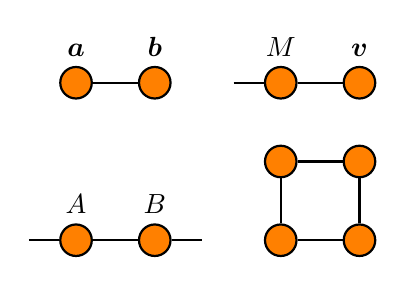
\begin{tikzpicture}
  \def\tensorsize{0.4cm}
  \def\verticalshift{2}
  \def\horizontalshift{2.6}
  \tikzstyle{tensor} = [circle, draw, fill=orange, thick, inner sep = 0pt, minimum size = \tensorsize]

  \begin{scope}[shift={(0,0)}]
    \node[tensor] (a) [label={$\bm{a}$}] at (0, 0) {};
    \node[tensor] (b) [label={$\bm{b}$}] at (1, 0) {};
    \draw[thick] (a) -- (b);
  \end{scope}

  \begin{scope}[shift={(\horizontalshift,0)}]
    \node[tensor] (M) [label={$M$}] at (0, 0) {};
    \node[tensor] (v) [label={$\bm{v}$}] at (1, 0) {};

    \draw[thick] (-1.5*\tensorsize, 0) -- (M);
    \draw[thick] (M) -- (v);
  \end{scope}

  \begin{scope}[shift={(0,-\verticalshift)}]
    \node[tensor] (A) [label={$A$}] at (0, 0) {};
    \node[tensor] (B) [label={$B$}] at (1, 0) {};

    \draw[thick] (-1.5*\tensorsize, 0) -- (A);
    \draw[thick] (A) -- (B);
    \draw[thick] (B) -- (1.6, 0);
  \end{scope}

  \begin{scope}[shift={(\horizontalshift,-\verticalshift)}]
    \node[tensor] (A) at (0, 0) {};
    \node[tensor] (B) at (1, 0) {};
    \node[tensor] (C) at (1, 1) {};
    \node[tensor] (D) at (0, 1) {};

    \draw[thick] (A) -- (B);
    \draw[thick] (B) -- (C);
    \draw[thick] (C) -- (D);
    \draw[thick] (D) -- (A);

  \end{scope}
  %\begin{scope}[shift={(2,0)}]
    %\node[tensor] (M) [label={$M_{i j}$}] at (0, 0) {};
    %\draw[thick] (M) -- (-1.5*\tensorsize, 0);
    %\draw[thick] (M) -- (1.5*\tensorsize, 0);
  %\end{scope}

  %\begin{scope}[shift={(4, 0)}]
    %\node[tensor] (T) [label={$T_{i j k}$}] at (0, 0) {};
    %\draw[thick] (T) -- (-1.5*\tensorsize, 0);
    %\draw[thick] (T) -- (1.5*\tensorsize, 0);
    %\draw[thick] (T) -- (0, -1.5*\tensorsize);
  %\end{scope}



\end{tikzpicture}
\end{document}
